\newpage
\section{Computer Abstractions and Technology}

\subsection{Introduction}

\subsubsection{History of Computers}

\begin{enumerate}
    \item Pre-computer: 计数的辅助工具
    \begin{enumerate}
        \item The First Mechanical Calculating Machine
        \item Turing Machine: 计算与跳转
        \item First Electronic Digital Computing Device: 
        \item First General-Purpose Electronic Computers
    \end{enumerate}
    \item First Generation: Vacuum Tubes (真空管)
    \begin{enumerate}
        \item von Neumann Architecture: 计算与储存分离, 数据与指令保存在同一个储存器. 但遇到数据密集型此架构会有限制. 
        \begin{figure}[H]
            \centering
            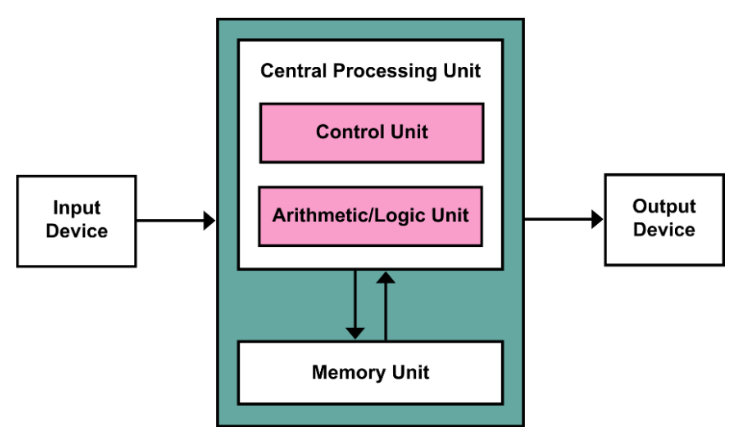
\includegraphics[width=0.309\textwidth]{CO1/von Neumann Architecture}
            \caption{von Neumann Architecture}
        \end{figure}
        
        \item Analog Computing: 
        \item Digital Computing: 
    \end{enumerate}
    \item Second Generation: Transistors (晶体管)
    \begin{enumerate}
        \item IBM
    \end{enumerate}
    \item Third Generation: Integrated Circuits (集成电路)
    \item Fourth Generation: Microprocessors
    \begin{enumerate}
        \item The First Modern Personal Computer
        \item Commercial Personal Computer
        \item RISC Architecture
    \end{enumerate}
    \item Fifth Generation:
    \begin{enumerate}
        \item Quantum Computer
        \item Neuromorphic Computer
    \end{enumerate} 
\end{enumerate}

\subsection{Computer Organization}

\begin{enumerate}
    \item 电子化的实现方式
    \item 有指令集
    \item 可执行指令
    \item 可存储指令与数据
    \item 计算能力上是图灵完全的
\end{enumerate}

\subsubsection{Decomposability of Computer Systems}

\begin{figure}[H]
    \centering
    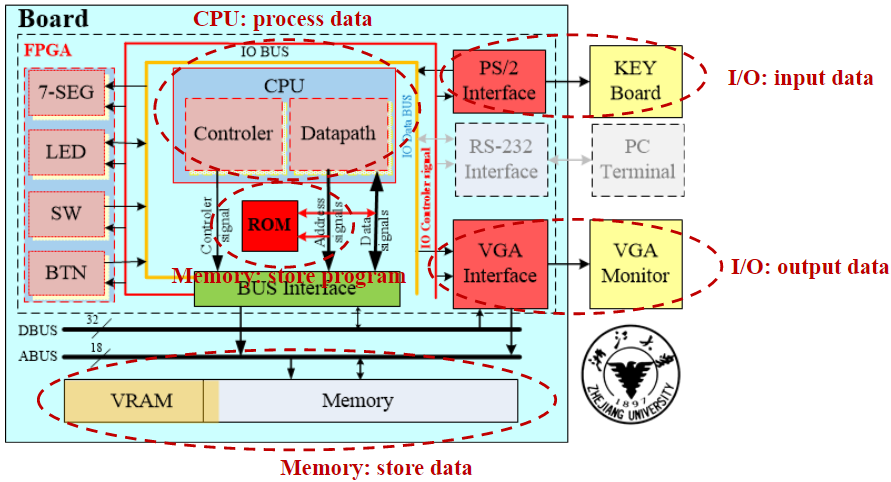
\includegraphics[width=0.309\textwidth]{CO1/Five Classic Components of Hardware}
    \caption{Five Classic Components of Hardware}
\end{figure}


Hardware: 
\begin{itemize}
    \item CPU
    \begin{itemize}
        \item Control unit
        \item Datapath
        \begin{itemize}
            \item Path: multiplexors
            \item ALU: adder, multiplier
            \item Registers
            \item $\cdots$
        \end{itemize}
    \end{itemize}
    \item Memory: 层级化
    \item I/O interface
    \begin{itemize}
        \item Input: keyboard
        \item Bidirectional: RS-232, USB
        \item Output: VGA, LCD
    \end{itemize}
\end{itemize}

Software: 
\begin{itemize}
    \item Application software (应用软件): word, PPT, office
    \item System software
    \begin{itemize}
        \item Operation system (操作系统): Linux, macos
        \item Compiler (编译器): GCC
        \item Firmware (Driver software): 网卡驱动 
    \end{itemize}
\end{itemize}

指令集体系架构: 连接硬件与软件 (抽象)

\subsubsection{From a High-Level Language to the Language of Hardware}

\begin{enumerate}
    \item Machine language
    \item Assembly language
    \item High-level programming language
\end{enumerate}

\subsection{How to Build Processors}
了解一下
\subsubsection{Integrated Circuits (ICs)}
主板核心

\begin{enumerate}
    \item Manufacturing ICs
    \begin{figure}[H]
        \centering
        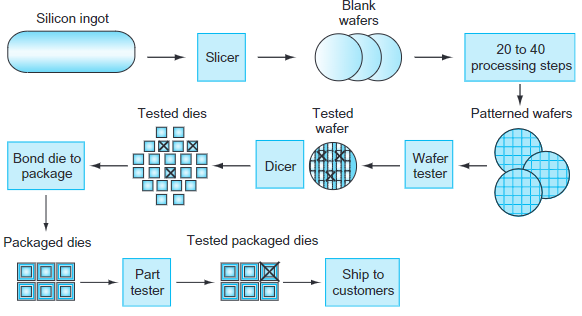
\includegraphics[width=0.48\textwidth]{CO1/The chip maunfacturing process}
        \caption{The chip maunfacturing process}
    \end{figure}
    \item Cost: Yield, proportion of working dies per wafer. 
\end{enumerate}

\subsubsection{Challenges of the Processor}
\begin{enumerate}
    \item 内存墙
    \item 功耗墙
    \item 工艺发展限制
\end{enumerate}

\subsection{Computer Design:Performance and Idea}

\subsubsection{Response Time and Throughput}
\begin{itemize}
    \item Response/execution time: 响应时间 (one task)
    \item Throughput (bandwidth): 吞吐率 (total work)
\end{itemize}

\subsubsection{Relative Performance}
Define Performance=1/Execution

e.g. 10s on A, 15s on B, A is $\frac{\frac{1}{10}}{\frac{1}{15}}=1.5$ times faster than B. 

\subsubsection{Measuring Execution Time}
\begin{itemize}
    \item Elapsed time: Total response time, including all aspects. 
    \item CPU time: Time spent processing a given job. 
    \begin{align*}
        \text{CPU Time}&=\text{CPU Clock Cycles} \times \text{Clock Cycle Time}\\
        &=\frac{\text{CPU Clock Cycles}}{\text{Clock Rate}}
    \end{align*}
    \item Clock period: duration of a clock cycle. 
    
    e.g. $250\mathrm{ps}=0.25\mathrm{ns}=250\times 10^{-12}\mathrm{s}$
    \item Clock frequency: cycles per second. 
    
    e.g. $4.0\mathrm{GHz}=4000\mathrm{MHz}=4.0\times 10^9\mathrm{Hz}$
\end{itemize}

\subsubsection{Instruction Count and CPI}

\scalebox{0.80}{ %缩小整个内容
	\parbox{0.55\textwidth}{ %延长内容的水平宽度
    \begin{align*}
        \text{Clock Cycles}=&\text{Instruction Count} \times \text{Cycles per Instruction (CPI)}\\
        \text{CPU Time} =& \text{Instruction Count} \times \text{CPI} \times \text{Clock Cycle Time}\\
        =&\frac{\text{Instruction Count} \times \text{CPI}}{\text{Clock Rate}}
    \end{align*}
	}
}

Instruction Count for a program: Determined by program, ISA and compiler. 

Average cycles per instruction: Determined by CPU hardware. If different instructions have different CPI, average CPI affected by instruction mix. 

CPI in More Detail: 
If different instruction classes take different numbers of cycles
\begin{align*}
    \text{Clock Cycles}=\sum_{i=1}^n (\text{Instruction Count}_i \times \text{CPI}_i)
\end{align*}

Weighted average CPI: 
\begin{align*}
    \text{CPI}=&\frac{\text{Clock Cycles}}{\text{Instruction Count}}\\
    =&\sum_{i=1}^n \left( \text{CPI}_i \times \frac{\text{Instruction Count}_i}{\text{Instruction Count}} \right)
\end{align*}
$\displaystyle \frac{\text{Instruction Count}_i}{\text{Instruction Count}} $ is relative frequency. 

\subsubsection{Performance Summary}
\begin{align*}
    \text{CPU Time}=\frac{\text{Instruction}}{\text{Program}}\times \frac{\text{Clock cycles}}{\text{Instruction}}\times \frac{\text{Seconds}}{\text{Clock cycle}}
\end{align*}

Performance depends on
\begin{itemize}
    \item Algorithm: affects IC, possibly CPI
    \item Programming language: affects IC, CPI
    \item Compiler: affects IC, CPI
    \item Instruction set architecture: affects IC, CPI, $\text{T}_c$
\end{itemize}

\subsubsection{Power Trends}
In CMOS IC technology

\scalebox{0.88}{ %缩小整个内容
	\parbox{0.5\textwidth}{ %延长内容的水平宽度
    \begin{align*}
        \text{Dynamic Power}=\text{Capacitive load}\times \text{Voltage}^2 \times \text{Frequency}
    \end{align*}
	}
}

\subsubsection{Multiprocessors}
More than one processor per chip. Requires explicitly parallel programming. 

\subsubsection{Benchmark}
\begin{enumerate}
    \item SPEC CPU Benchmark: Programs used to measure performance, supposedly typical of actual workload. e.g. SPEC CPU2006. 
    \item SPEC Power Benchmark: Power consumption of server at different workload levels. 
    \begin{itemize}
        \item Performance: ssj\_ops/sec
        \item Power: Watts (Joules/sec)
    \end{itemize}
\end{enumerate}

\subsubsection{Pitfall: Amdahl’s Law}
Improving an aspect of a computer and expecting a proportional improvement in overall performance. 
\begin{align*}
    T_{\text{improved}}=\frac{T_{\text{affected}}}{\text{improvement factor}}+T_{\text{unaffected}}
\end{align*}

Corollary: make the common case fast. 

\subsubsection{Pitfall: MIPS as a Performance Metric}
MIPS: Millions of Instructions Per Second
\begin{align*}
    \text{MIPS}=&\frac{\text{Instruction Count}}{\text{Execution Time}\times 10^6}\\
    =& \frac{\text{Instruction Count}}{\frac{\text{Instruction Count}\times \text{CPI}}{\text{Clock Rate}}\times 10^6} \\
    =&\frac{\text{Clock Rate}}{\text{CPI}\times 10^6}
\end{align*}

\subsection{Eight Great Ideas}
\begin{enumerate}
    \item Design for Moore’s Law (设计紧跟摩尔定律)
    \item Use Abstraction to Simplify Design (采用抽象简化设计)
    \item Make the Common Case Fast (加速大概率事件)
    \item Performance via Parallelism (通过并行提高性能)
    \item Performance via Pipelining (通过流水线提高性能)
    \item Performance via Prediction (通过预测提高性能)
    \item Hierarchy of Memories (存储器层次)
    \item Dependability via Redundancy (通过冗余提高可靠性)
\end{enumerate}
